\pattern{Command}
\begin{summary}
    The {\bf command} design pattern is a behavioral design pattern that is
    used for objects to issue requests/commands to receiver objects, while
    maintaining modular design. 
    
    It does this by encapsulating a command as an object type, thus allowing
    multiple operations of varying complexity that can be performed on a
    receiver. 

    It seeks to solve the problem of supporting potentially thousands of
    commands, for many different receiver objects, without hard-coding in
    commands to specific receivers. 
\end{summary}

\subsubsection{Use-case}

Hard-coding actions is very space inefficient because you will need to support
two different classes to perform the same operation if, for example, you are
turning both a radio and a TV on. 

The command pattern solves this by decoupling the command caller (the invoker)
from the object that knows how to perform the request. Thus, the invoker has no
knowledge of who will perform a given task. In the TV example, there would be 1
command called {\sc turnOn} which can be called on both TV and Radio types
depending on what receiver is in the concrete command.

Concrete commands consist of receiver object interface to perform actions
on different receiver objects.

\comparison{\begin{itemize}
        \item Complexity: The client could be oblivious to the implementation. 
            It does not care about the related problems of the task such as
            user-server synchronization and security, and it also has no idea
            about the actual business process. 
        \item Evolvability: The structure can be easily extended, due to each
            command is an independent class.
        \item Complexity: the history stack feature helps the invoker to trace
            back previous commands, and execute undo operations.
        \item Low coupling: the invoker has no knowledge of who will perform a
            task, allowing for loose coupling, and making it easier to add new
            commands without modifying existing code.
    \end{itemize}
}{\begin{itemize}
        \item Efficiency: will be very bulky if the client knows the business
            process very well, or the process is very simple. This will be a
            major restriction of a real-time system. 
        \item Complexity: because each command is a separate class, the
            extension of the system will make the code management difficult.
        \item Complexity: Each command fulfills an interface of a class, thus
            every subclass has to implement all of the interfaces that relate
            to. This also generates a lot of redundant code.
    \end{itemize}
}% END comparison

\begin{nfps}
\item[Extensibility] Command Design Pattern is perfect for
    achieving loose Coupling and high Cohesion. Invoker has a Command Interface
    not the concrete commands, which means invoker is loosely coupled with the
    concrete commands. New Concrete commands can be easily created under
    interface and invoker, with no need to know about the new concrete
    commands.  When new receivers are added, invokers don't need to know all
    the details.  Invoker just needs command interface for calling the concrete
    commands.

\item[Maintainability] The Command Pattern has high cohesion this means that
    classes now have well-defined, narrow responsibilities. Each concrete
    command class focuses on specific action on the receiver. It is much easier
    to maintain as these classes are less frequently changed. Each concrete
    command consists of receiver interface, which can be used to perform
    specific action on the receiver object.

\item[Scalability] Different receivers and commands can be added, which means
    more functionality can be added without affecting original workflow. When
    new receiver objects are created, new concrete commands are created which
    do not affect old concrete commands. As a result, original functionality is
    not affected. Applications using command design pattern have an advantage
    of high scalability, where new objects are created to achieve new
    functionality.

\end{nfps}

\begin{center}
    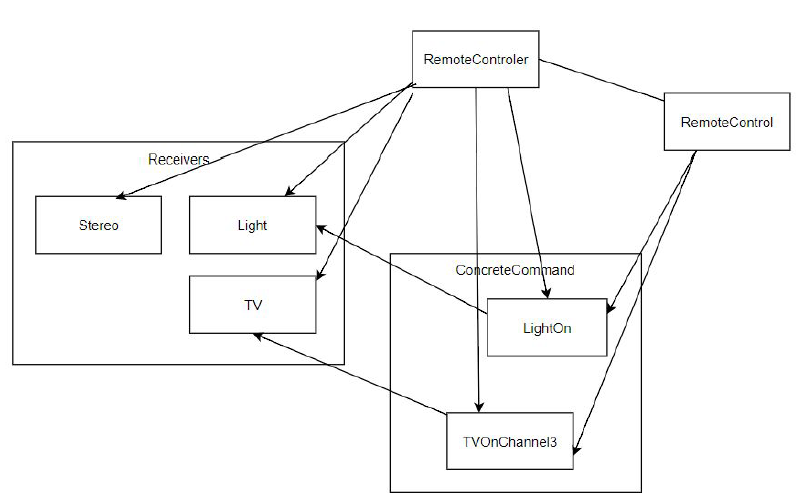
\includegraphics[width=0.4\textwidth]{./command}
    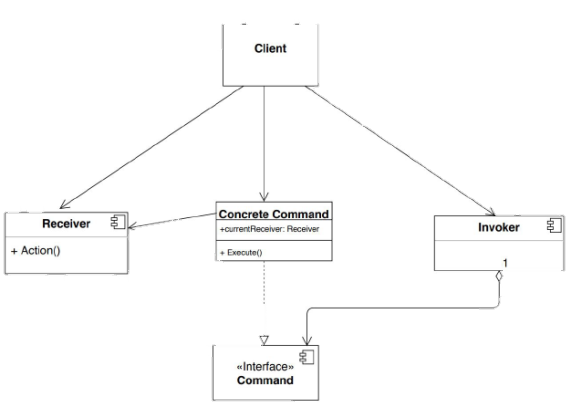
\includegraphics[width=0.4\textwidth]{./command2}
\end{center}
